\item {\bf Learning Imbalanced Dataset}

In this problem, we study how to learn a classifier from an imbalanced dataset, where the marginal distribution 
of the classes/labels are imbalanced. Imbalanced datasets are ubiquitous in real-world applications. For example, 
in the spam detection problem, the training dataset usually has only a small fraction of spam emails 
(positive examples) but a large fraction of ordinary emails (negative examples). 
For simplicity, we consider binary classification problem where the labels are in $\{0,1\}$ 
and the number of positive examples is much smaller than the number of negative examples.

\textbf{Note: We will be using the logistic regression classifier defined in problem 1. If you haven't done so 
already, finish implementing the Logistic Regression class in src-linear/submission/logreg.py}

\textbf{Code Deliverables}
\begin{itemize}
    \item \texttt{src-imbalanced/submission.py}
    \item \texttt{src-imbalanced/logreg.py} \textbf{   **Copied over from src-linear/submission/logreg.py}
\end{itemize}

\begin{enumerate}
    \input{03-imbalanced/01-evaluation}

    \item \points{3b} \textbf{Coding problem: vanilla logistic regression}

First, we use the vanilla logistic regression to learn an imbalanced dataset. For the rest of the question, we will use the dataset and starter code provided in
the following files:
%
\begin{center}
	\begin{itemize}
		\item	\texttt{src-imbalanced/{train,validation}.csv}
		\item   \texttt{src-imbalanced/submission.py}
	\end{itemize}
\end{center}

Please complete |apply_logistic_regression| and |calculate_accuracies| functions.

Each file contains $n$ examples, one example $(x^{(i)}, y^{(i)})$ per row. $x$ is two-dimensional, i.e., the $i$-th row contains columns $x^{(i)}_1\in\Re$,
$x^{(i)}_2\in\Re$, and $y^{(i)}\in\{0, 1\}$. Let $\calD=\{(x^{(i)}, y^{(i)})\}_{i=1}^n$ be our training dataset. $\calD$ has $\rho n$ examples with label 1 and $(1-\rho)n$ with label 0. In the dataset we constructed, $\rho=1/11$.

You will train a linear classifier $h_{\theta}(x)$ with average empirical loss for logistical regression, where $h_\theta(x)=g(\theta^T x), g(z)=1/(1+e^{-z})$, similar to Problem 1 Part a:
\begin{align*}
J(\theta) = -\frac{1}{\nexp} \sum_{i=1}^\nexp \left(y^{(i)}\log(h_{\theta}(x^{(i)}))
+  (1 - y^{(i)})\log(1 - h_{\theta}(x^{(i)}))\right), 
\end{align*}

After obtaining the classifier, compute the classifier's accuracy ($A$), balanced accuracy ($\overline{A}$), accuracies for the two classes ($A_0, A_1$) on the validation dataset. You are expected to observe that the minority class (positive class) has significantly lower accuracy than the majority class. 

The output plot should look similar to the following (no plot submission is required):

\begin{figure}[H]
	\centering
	\vspace{2mm}
	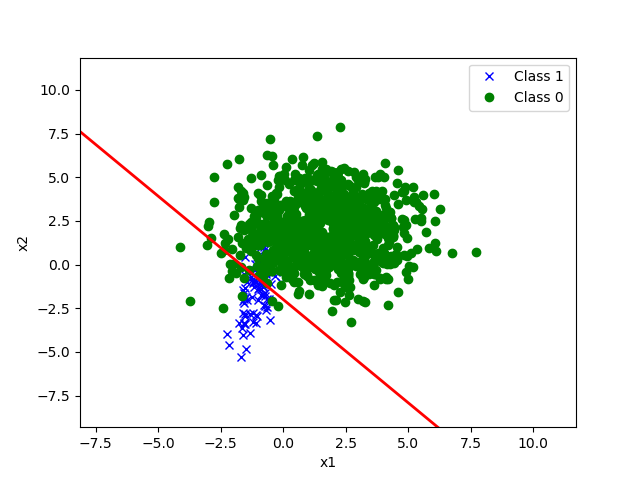
\includegraphics[width=0.5\linewidth]{03-imbalanced/imbalanced_naive_pred.png}
	  \caption{Validation set with $x_1$ on the horizontal axis and $x_2$ on
	  the vertical axis. The decision boundary obtained by your model (i.e, line corresponding to model's predicted probability = 0.5). Visual impaired students can access the corresponding desmos plot \href{https://www.desmos.com/calculator/6q35atu7ti}{here}}
  \end{figure}


    \input{03-imbalanced/03-proof}

    \item \points{3d} \textbf{Coding problem: re-weighting minority class}

In \texttt{src-imbalanced/submission.py}, implement the logistic regression algorithm on $\calD'$.  Compute and report the classifier's accuracy ($A$), balanced accuracy ($\overline{A}$), accuracies for the two classes ($A_0, A_1$) on the validation dataset. You are expected to see that the accuracy of minority class (class 1) improved significantly whereas that of the majority class dropped compared to vanilla logistic regression. However, the balanced accuracy is significantly greater than that of the vanilla logistic regression. 

Please adjust the |apply_logistic_regression| you worked with in 3b to capture the reweighted minority class solution. 
Then fill in the |upsample_minority_class| function. 

The output plot should look similar to the following (no plot submission is required):

\begin{figure}[H]
	\centering
	\vspace{2mm}
	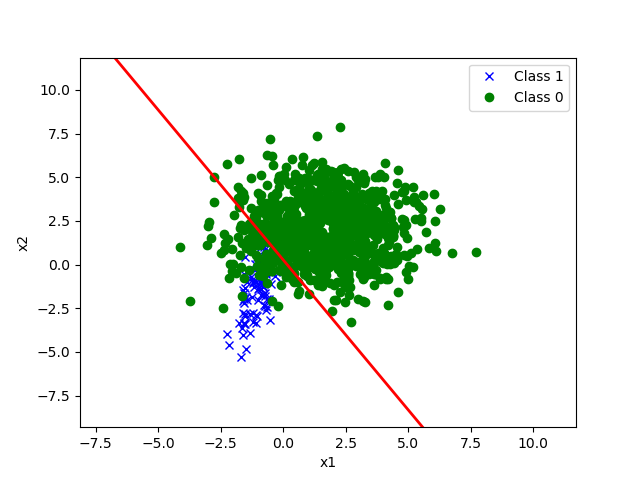
\includegraphics[width=0.5\linewidth]{03-imbalanced/imbalanced_upsampling_pred.png}
	  \caption{Validation set with $x_1$ on the horizontal axis and $x_2$ on
	  the vertical axis. The decision boundary obtained by your model (i.e, line corresponding to model's predicted probability = 0.5). Visual impaired students can access the corresponding desmos plot \href{https://www.desmos.com/calculator/yzewr1djk7}{here}}
  \end{figure}
\end{enumerate}
